\section*{Part 5：Dataset B 與跨資料集歸納}
\vspace{-0.5em}

\q{19}{Digits 資料摘要。}
Digits 有 1797 筆、64 個像素特徵與 10 類；各類筆數依 0--9 為 178、182、177、183、181、182、181、179、174、180，固定切分為 1437/360。相較 Dataset A，Digits 樣本較多、類別由 2 增至 10，且特徵是結構化的 $8\times8$ 灰階像素（0--16），而 A 是 30 個量測尺度差異很大的連續醫療特徵。

\q{20}{比較基準。}
Dataset B 不另外進行超參數搜尋，沿用 Part 2 的 baseline 模型設定。依題目要求，kNN 與 SVM 先標準化，其餘模型使用原始特徵；StandardScaler 只在 Dataset B 的訓練集上 fit。所有模型仍使用相同的資料切分。

\q{21}{五模型結果與最佳模型混淆矩陣。}
\begin{center}
\compacttable
\begin{tabular}{cllrr}
\toprule
排名 & 分類器 & 設定 & Accuracy & Macro-F1 \\
\midrule
1 & SVM & Scaled, RBF, $C=1$ & 0.9750 & 0.9748 \\
2 & kNN & Scaled, $k=5$ & 0.9639 & 0.9634 \\
3 & Random Forest & Raw, 200 trees & 0.9639 & 0.9634 \\
4 & Decision Tree & Raw, seed 42 & 0.8222 & 0.8209 \\
5 & Gaussian NB & Raw, defaults & 0.8111 & 0.8137 \\
\bottomrule
\end{tabular}
\end{center}
排名仍先依 Macro-F1、再依 Accuracy。SVM 在 360 筆 test 中正確 351 筆；錯誤主要出現在 8 被判為 1/4，以及 9 被判為 6/7。

\begin{center}
\begin{minipage}{0.72\linewidth}
\centering
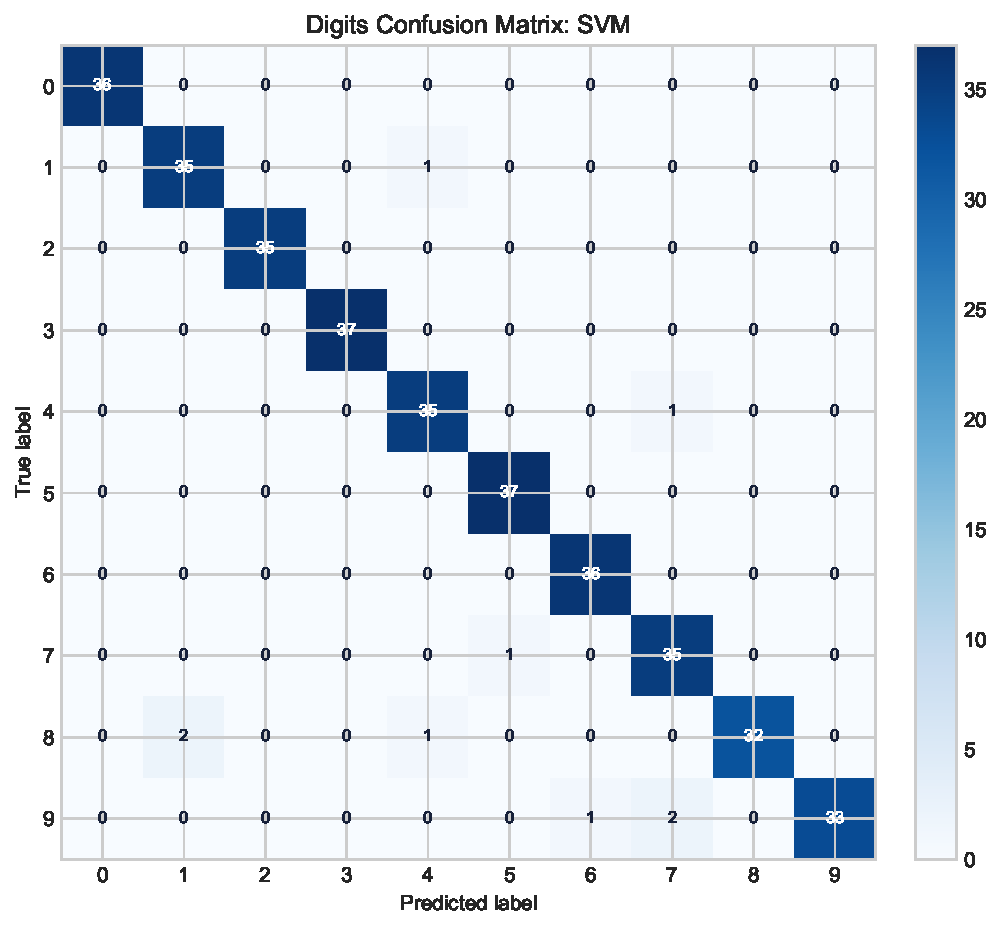
\includegraphics[width=0.67\linewidth]{digits_confusion_matrix.pdf}
\par\small Figure 3：Dataset B 最佳模型 SVM 的混淆矩陣；列為真實類別、欄為預測類別。
\end{minipage}
\end{center}

\q{22}{跨資料集名次。}
Dataset A 的 raw baseline 以 Random Forest 第一、Gaussian NB 第二、SVM 第三；到了 Dataset B，SVM 升至第一，kNN 第二，而 Gaussian NB 降到第五。Digits 的像素特徵與多類別結構，可能更適合 SVM 與 kNN 的判別方式；Gaussian NB 的條件獨立假設則較難描述像素之間的關係。單棵決策樹在這組資料上的表現也明顯較低。需要注意的是，Dataset B 的 kNN、SVM 依題目規定使用了標準化，因此排名差異不能完全歸因於資料集本身。

\textcolor{accent}{\textbf{五分類器特性歸納表。}}
\begin{center}
\scriptsize
\rowcolors{2}{lightrow}{white}
\begin{tabularx}{\linewidth}{lC{1.7cm}Y Y Y}
\toprule
模型 & Scaling 敏感？ & 重要參數/特性 & 本作業優點 & 本作業限制 \\
\midrule
Decision Tree & 否；A 分數不變 & max\_depth；單樹規則可讀 & 可解釋、免 scaling & A final F1 .8907；B 僅 .8209，變異較大 \\
Random Forest & 否；A 分數不變 & n\_estimators；多樹投票 & A raw 第一 .9526；B .9634 & 計算與記憶體高於單樹，整體規則較難讀 \\
kNN & 是；A +.0460 F1 & $k$、距離；延遲式學習 & A final .9713；B .9634 & 預測需保留/搜尋訓練樣本，尺度影響大 \\
Gaussian NB & 本次未 scaling & var\_smoothing；條件獨立高斯 & A raw 第二 .9337；快速簡單 & B 最後 .8137，假設與像素相依性不合 \\
SVM & 是；A +.0582 F1 & $C$、RBF kernel；margin & A final .9719；B 第一 .9748 & scaling/調參重要，決策邊界不易解釋 \\
\bottomrule
\end{tabularx}
\end{center}

\q{23}{是否存在 universally best classifier？（200--300 字）}
\label{q23text}
我認為沒有一種分類器能在所有資料集上都保持最佳表現。乳癌資料的原始特徵中，Random Forest 以 Macro-F1 0.9526 排名第一，但標準化後 SVM 升至 0.9812；Digits 則由 SVM 以 0.9748 居首，Random Forest 為 0.9634，顯示模型表現會受到資料特性與前處理方式影響。SVM 與 kNN 對 scaling 明顯敏感，樹模型則完全不變。Random Forest 需要訓練多棵樹，通常比單棵樹耗費更多資源；單棵樹較容易解釋，但本次分數較低。SVM 表現不錯，決策過程卻比較難直觀說明。kNN 訓練便宜，推論卻須保留並搜尋樣本。此外，類別數、樣本量、特徵尺度與資料結構不同，都可能改變模型的相對優勢。因此，選擇分類器時應參考交叉驗證結果，也要考慮解釋性、運算成本及實際應用需求。

\q{24}{實務推薦。}
Dataset A 我會選擇經交叉驗證選出的 RBF SVM（標準化、$C=10$），其最終 Macro-F1 為 .9719，在三個有進行選參的模型中最高。但醫療資料也重視判斷依據，若需要更容易說明的模型，可以考慮 Random Forest，並搭配特徵重要度分析。Dataset B 則推薦標準化後的 SVM（$C=1$），Accuracy 為 .9750、Macro-F1 為 .9748，360 筆測試資料中僅錯 9 筆。若更重視省去標準化流程，也可以考慮 Macro-F1 為 .9634 的 Random Forest。
